\documentclass[twocolumn]{article}
\usepackage{fullpage}
%%\usepackage{amsmath}
%%\usepackage{amssymb}
\usepackage{amsthm}
%\usepackage{hyperref}
\usepackage{algpseudocode}
%%\usepackage{ulem}
%%\usepackage{setspace}
\usepackage{graphicx}
\usepackage{subcaption}
%%\usepackage{phonetic}
%%\usepackage{synttree}

%\setlength{\columnsep}{14pt}

%\usepackage{rotating}
\usepackage{mathspec}
%\usepackage{fouriernc}
%\usepackage[T1]{fontenc}
%\usepackage[veryoldstyle]{kpfonts}

\newfontfamily\oldestyle{Slavkappen}

\setallmainfonts{OldNewspaperTypes}

%\usepackage{titlesec}
%\titleformat{\section}
%  {\normalfont\oldestyle\Large\bfseries}
%  {\thesection}{1em}{}


\renewcommand\exists{\reflectbox{E}}
\renewcommand\forall{\raisebox{\depth}{\rotatebox{180}{A}}}

%\newcommand{\longs}{\hspace{-1.5pt}$\int$\hspace{-2.5pt}}
\theoremstyle{plain}  % Italic body text
  \newtheorem{defn}{Definition}
  \newtheorem{thm}{Theorem}
  \newtheorem{lemma}{Lemma}
\theoremstyle{definition}  % Roman body text
  \newtheorem{proc}{Procedure}
\theoremstyle{remark}  % Italic header, roman body text
  \newtheorem{rem}{Remark}
  \newtheorem{cond}{Condition}


  \title{\em \huge A CONSTRVCTIVE SOLVTION TO THE K\"ONIGS-PITTSBVRGH BRIDGE PROBLEM}
\author{Greg HANNEMAN\\
	Language Enthusiast and Errant Scribbler
	%\footnote{and Salaried Employee now too!}
	\\
        Carnegie Mellon Vniversity
	\and
	Benj. BLVM \\
	Light Cone Sedentarian \\
	Carnegie Mellon Vniversity}
\date{}
\pagestyle{empty}


\begin{document}
%\normalem

\maketitle
\pagestyle{empty}
\thispagestyle{empty}

\section*{ABSTRACT.}
	We walked across a bunch of bridges one day.

% Format this paper to look like an old-style cramped math paper from like the '50s.  All math, no text, very dense.


\section*{\S 1..... BACKGROVND.}

Figure \ref{fig:koenigs} and Definition \ref{Def-Konigs} state the well-studied K\"onigsberg Bridge Problem \cite{original}. % http://math.dartmouth.edu/~euler/docs/originals/E053.pdf

\begin{defn} \label{Def-Konigs}
	The K\"onigsberg Bridge Problem (KBP). % Refers to ``the figure''

Regiomonti in Borussia esse insulam A {\em der Kneiphof} dictam, fluviumque eam cingentem in duos dividi ramos, quemadmodum ex figura videre licet: ramos uero huius fluvii septem instructos esse pontibus, $a$, $b$, $c$, $d$, $e$, $f$, et $g$.  Circa hos pontes iam ista proponebatur quaestio, num quis cursum ita instituere queat, ut per singulos pontes semel et non plus quam semel transeat.
\end{defn}

According to the best modern scholarship, it is thought that this passage reads as follows.

\begin{quote}
	,,At K\"onigsberg in Prussia there is an island A (Kneiphof), and flowing around it is divided into two branches, as shown in the figure; and the branches of the river, seven bridges, however, of this, \$a\$, \$B\$, \$C\$, \$d\$, \$e\$, \$F\$, and \$G\$. Already presented to him, the question concerning these bridges is, the course to be instructed so to whether a person may be able to, and not more than once in order to pass one by one the bridges honey themselves.''
\end{quote}

\begin{figure}[h]
\centering
	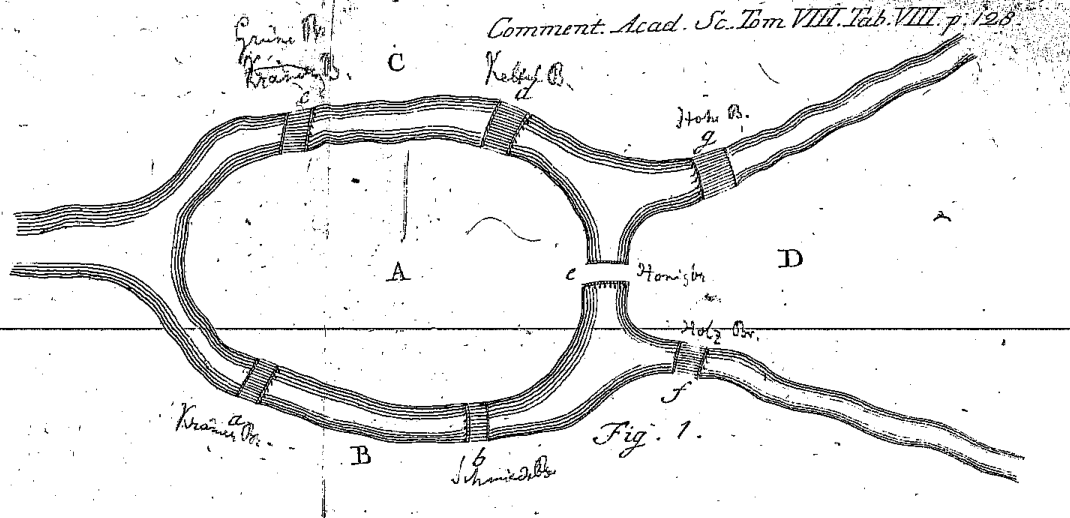
\includegraphics[width=0.48\textwidth]{koenigsburg.pdf}
	\caption{Kaliningrad, Russia (colloq.); better Known in the Formal Literature as K\"onigsberg, Prussia}
	\label{fig:koenigs}
\end{figure}

The criteria expressed in Definition \ref{Def-Konigs} have been generalized to arbitrary geographical topologies. % TODO: cite?
Of extreme local interest is the instance derived from the city of Pittsburgh, Pennsylvania, V.S.A., as Definition \ref{Def-KonigsPgh}.

\begin{defn} \label{Def-KonigsPgh}
	The K\"onigs-Pittsburgh Bridge Problem (KPBP).

Cross every pedestrian-navigable trans-Three-River bridge with at least one endpoint in the city of Pittsburgh, exactly once, to be accomplished during one continuous circuit.
\end{defn}

This article presents a constructive proof for the existence of a solution to KPBP. Furthermore, while most prior work \cite{wikipedia} has largely focused on theoretical analysis of KBP variants based on graph theory, here we additionally offer a more practical approach based on ambulation theory.

\section*{\S 2..... FORMALIZATION.}

The formal statement of KBP inquires after the existence of an Eulerian path on a graph representing K\"onigsberg, with one node to represent each of the landmasses connected by various edges (bridges). In KPBP we simply change the graph to represent the topology of our home city (Figure \ref{fig:map}).\footnote{The astute observer will note that no edge among our formalism represents the $32^{\text{nd}}$ street bridge. During the progress of our research, this bridge did not exist due to construction, and hence is omitted. If added to the graph (call it KPBP'), it is known that a non-cyclic solution exists, but a constructive proof is left to future work.}

\begin{figure}[t]
\centering
	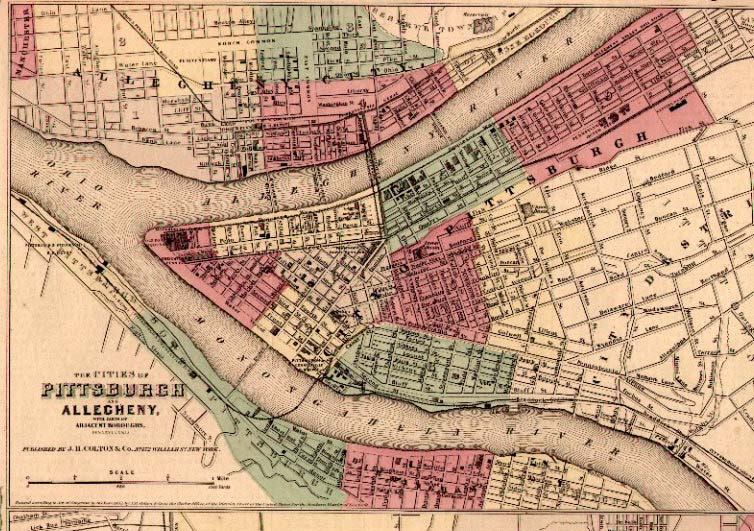
\includegraphics[width=0.35\textwidth]{1859pittsburgh.jpg}
	\caption{informal Diagram of the Topology of Pittsburgh, Pennsylvania as defined by its Bridges and Rivers.}
	\label{fig:map}
\end{figure}

\begin{figure}[t]
\centering
	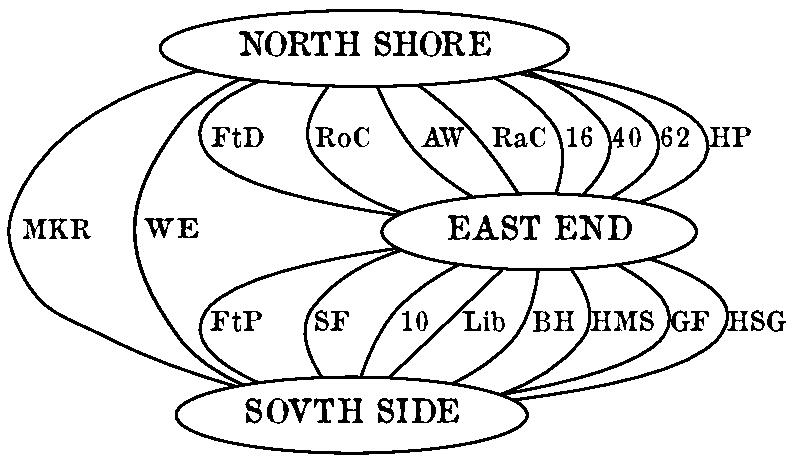
\includegraphics[width=0.48\textwidth]{topology.pdf}
	\caption{Formalization of Figure \ref{fig:map}.}
	\label{fig:topo}
\end{figure}

Vnlike KBP, in KPBP we require an Eulerian circuit, rather than an Eulerian path.
Recent developments in ambulation theory have shifted the common wisdom towards a preference for the use of circuits over paths in ambulatory proofs, as the circuit presents a more convenient practical application. (Put in more intuitive terms, the Eulerian circuit allows the bridge-walkers to sleep in their own beds the following night, rather than being stranded across a river.) Fortunately, the topology we have selected for KPBP allows for such a solution..
% http://en.wikipedia.org/wiki/Eulerian_path

\section*{\S 3..... PROOF.}

\begin{thm}
The K\"onigs-Pittsburgh Bridge Problem is solvable.
\end{thm}

We present here a constructive solution to the problem, first given by Hanneman, Vangpat, and Blum (2012, Oct. 27, 5:15 a.m.--10:05 p.m.).  The full solution has length 35 miles and consumes approximately 17 hours of wall-clock time. We depict $R$ in two distinct styles, in a somewhat abbreviated form, in Table \ref{tab:solution} and Figure \ref{fig:solution}.

\begin{table}[b]
	\centering
	\small
	\begin{tabular}{ll}
	\begin{tabular}{|l|l|l|}
		\hline
		Node & Edge & Node \\
		\hline
		EE & HP & NS \\
		NS & 62 & EE \\
		EE & 40 & NS \\
		NS & 16 & EE \\
		EE & RaC & NS \\
		NS & AW & EE \\
		EE & RoC & NS \\
		NS & MKR & SS \\
		SS & WE & NS \\
		\hline
	\end{tabular}
	&
	\begin{tabular}{|l|l|l|}
		\hline
		Node & Edge & Node \\
		\hline
		NS & FtD & EE \\
		EE & FtP & SS \\
		SS & SF & EE \\
		EE & 10 & SS \\
		SS & Lib & EE \\
		EE & BH & SS \\
		SS & HMS & EE \\
		EE & GF & SS \\
		SS & HSG & EE \\
		\hline
	\end{tabular}
	\end{tabular}
	\caption{|R| = 35 mi.}
	\label{tab:solution}
\end{table}

Intermediate details may easily be filled in by following Procedure \ref{Proc-Walk}.

\begin{proc} \label{Proc-Walk}
Let $R$ be the given solution route for KPBP, $p$ be a position along it measured in miles from the start of $R$, and $\hat{r}_x$ be a unit vector in the direction of $R$ at position $x$.
\end{proc}

%%%%%%%%%%%%%
%\newpage
%\begin{turn}{1}
%\begin{minipage}{\textwidth}
%\begin{multicols}{2}

\begin{algorithmic}
\While{$p < $|R|}
    \State $\vec{d} \gets \mathrm{StepSize} \cdot \hat{r}_p$
    \State Walk($p, \vec{d}$)
    \State p $\gets$ p + ||$\vec{d}$||
\EndWhile
\end{algorithmic}

\begin{rem}
Some experimental determination will of course be necessary to arrive at the correct value of the StepSize variable.  We suggest a default value of 75 cm, to be adjusted upwards or downwards as personal height and local terrain require.
\end{rem}

\begin{lemma} \label{Lemma-Walk}
Walkability.

A point $p'$ along $R$ can be reached from point $p$ along $R$, following Procedure \ref{Proc-Walk}, assuming $p < p'$.

\end{lemma}
\begin{proof}
	Try it.
\end{proof}

\begin{figure}[t]
	\centering
	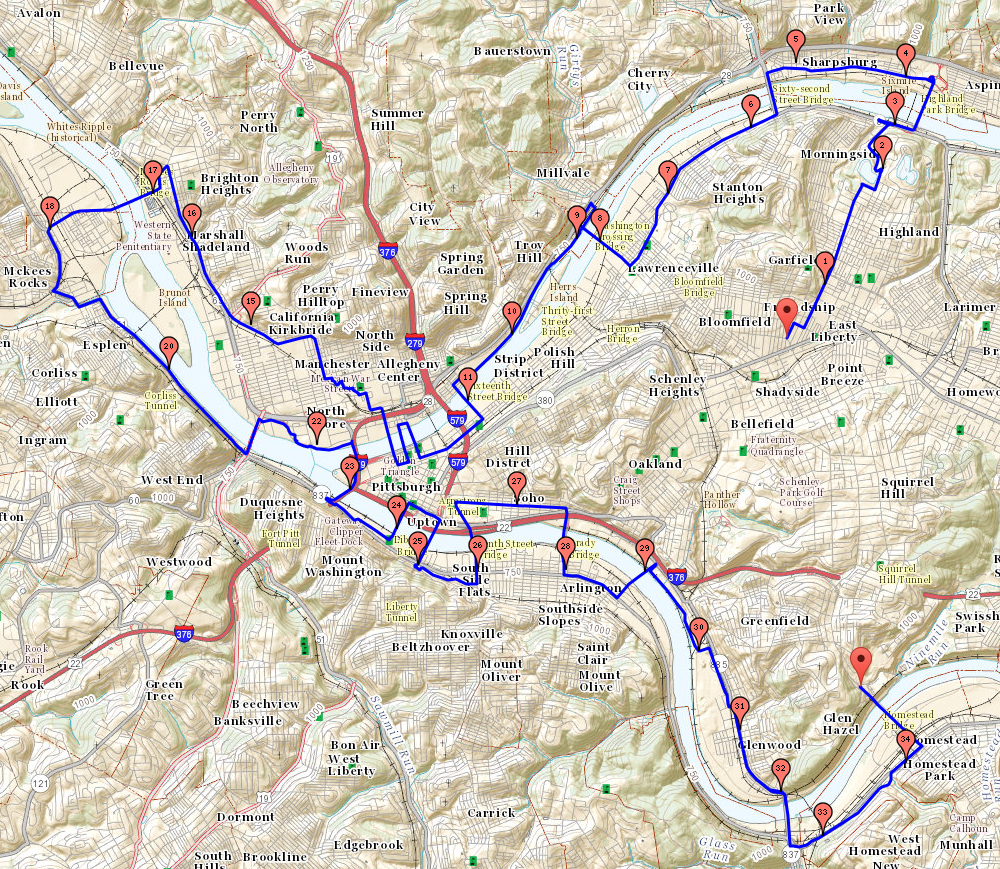
\includegraphics[width=0.48\textwidth]{solution.png}
	\caption{a cartographic Rendering of the Solution Route $R$.}
	\label{fig:solution}
\end{figure}

Lemma \ref{Lemma-Walk} thus establishes a ``modus ponens'' result for traversal of the route $R$ from its beginning (p = 0) to its end (p = |R|).  This is, however, a purely theoretical result.  We now show the practicability of the solution in an operational scenario via a number of satisfiable conditions.

\begin{cond}
	\label{cond:init}
Initialization.

Let $A$ be a set of attempting participants.  Then $a$ must be present at p = 0 \forall{}a $\in$ A.
\end{cond}

\begin{cond}
	\label{cond:prog}
Progression.

Let $B$ be a set of qualifying bridges such that the following are true \forall{}b $\in$ B:  (1) $b$ satisfies the bridge criteria from Definition \ref{Def-KonigsPgh}; (2) $b$ has defined 0 $\leq$ $p_b$ $\leq$ 35 on $R$.  Let $b_i$ be the $i$th ordered element of $B$, and let |B| = n.  Then C = \{$c_1, ..., c_n$\}, and $c_i$ = ($S_i, b_i$) iff some $S_i \subseteq A$ crosses $b_i$.
\end{cond}

\begin{cond}
	\label{cond:term}
Termination.

Let the set of ending participants $E \subseteq A$ = \{$a \in A\,|\, a \in S_i\ \forall{}i$\}.  Then the solution is successful iff $E \neq \emptyset$ and $e$ is present at p = 35 \forall{}e $\in$ E.
\end{cond}

\begin{lemma}
Satisfiability of Conditions.

Conditions 1--3 are satisfiable.
\label{lem:satisf}

\end{lemma}
\begin{proof}
	Set A = \{Alan, Ben, Dan, Greg, Keith\}. Note that Pr(x  awake at 5 a.m.) = $\epsilon$ \forall{}x $\in$ A. As long as $\epsilon$ > 0, $\epsilon^5$ > 0. \cite{what-is-epsilon}

Set B = \{Highland Park, 61st Street, 40th Street, 16th Street, 9th Street, 7th Street, 6th Street, McKees Rocks, West End, Fort Duquesne, Fort Pitt, Smithfield Street, Liberty, 10th Street, Birmingham, Hot Metal, Glenwood, Homestead Grays\}.
The bridge criteria of Definition \ref{Def-KonigsPgh} are satisfied $\forall{}b \in B$. Therefore the set $C$ of crossings may be freely constructed following $R$ from Figure \ref{fig:solution}.

Finally, set E = \{Alan, Ben, Greg\}.
The diagrams in Figure \ref{fig:photos} offer a visualization of these values for A, B, and E.

Since |E| = 3 > 0, this proves Lemma \ref{lem:satisf} and thus the successful instantiation of Conditions 1--3.  Together with Lemma \ref{Lemma-Walk}, this proves that $R$ is a navigable Eulerian circuit of the city of Pittsburgh.  Therefore a solution to the K\"onigs-Pittsburgh Bridge Problem exists.
\end{proof}

\section*{\S 4..... CONCLVSION.}


Vetere Konigsberg consequat pons (KBP) designat insulae urbem, flumina, pontes, qui in tali figuratione transiens per singulos semel iter unum non potest.
In hoc articulo quaestionis exposuimus accommodatio hodierna die ad oppidum Pittsburgh (KPBP).
Significat adaptationem ad profectum nostrum insignis civitas-in-es super duobus.

Vno modo, sicut KPBP est solubilis, offert mathematici nostram collationem incitamentum ad ire foris, et accipiam ab eo aliquid exercitium, quod hodie magis quam somnium, quod fieri non potest.
Deinde insuper offerebat speculativa ratio nos instruit etiam problema aedificant, qui probi ad ultimum pedes decem milia multa mala!

\renewcommand\refname{REFERENCES.}
\bibliographystyle{alpha}
\bibliography{sigbovik}

%%%%%%%%%%%%%
%\end{multicols}
%\end{minipage}
%\end{turn}
%\newpage

\begin{figure*}[b]
	\begin{tabular}{cc}
	\begin{subfigure}[b]{0.45\textwidth}
	\centering
	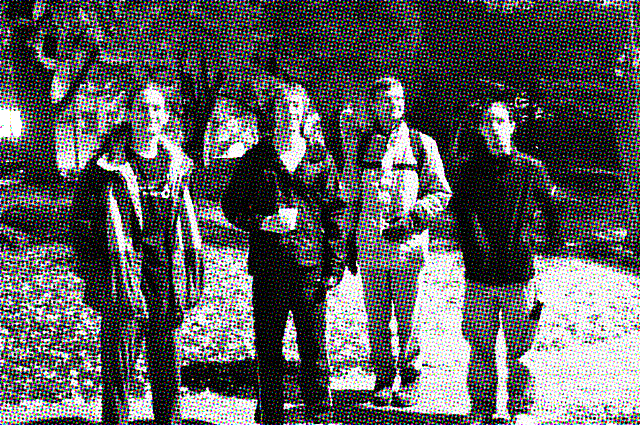
\includegraphics[width=\textwidth]{initialization.png}
	\caption{Condition \ref{cond:init}, Initialization.}
	\end{subfigure}
	&
	\begin{subfigure}[b]{0.45\textwidth}
	\centering
	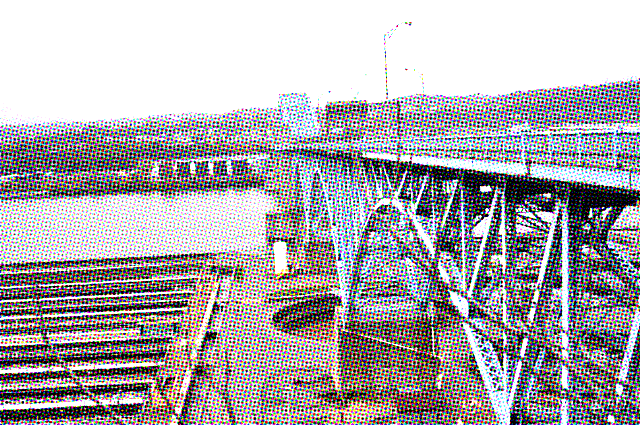
\includegraphics[width=\textwidth]{mckees.png}
	\caption{an example Member of the set $B$.}
	\end{subfigure}
	\\

	\begin{subfigure}[b]{0.45\textwidth}
	\centering
	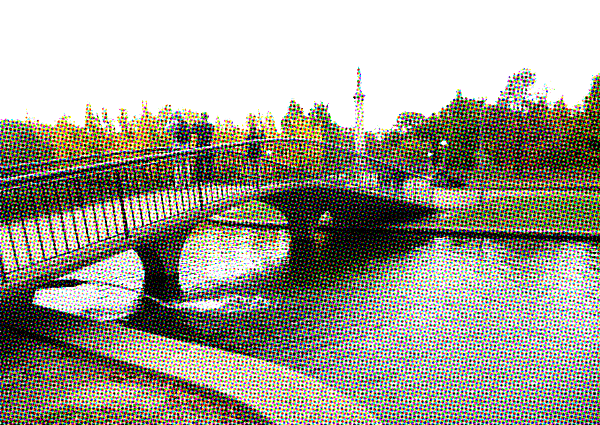
\includegraphics[width=\textwidth]{mini-koenigs.png}
	\caption{\exists b $\in$ R s.t. b $\not\in$ B.}
	\end{subfigure}
	&
	\begin{subfigure}[b]{0.45\textwidth}
	\centering
	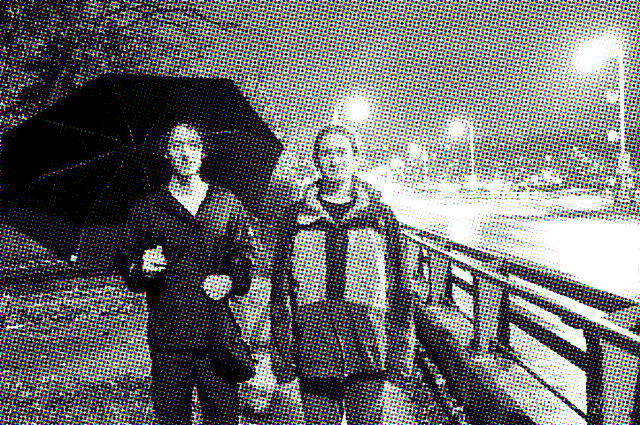
\includegraphics[width=\textwidth]{finish.png}
	\caption{Condition \ref{cond:term}, successful Termination.}
	\end{subfigure}

	\end{tabular}
	\caption{Satisfiability of Conditions. \cite{alanv}}
	\label{fig:photos}
\end{figure*}

\end{document}
